\cleardoublepage

\chapter{Simplified Framework Conceptual Scheme}
\begin{figure}[H]
    \centering
    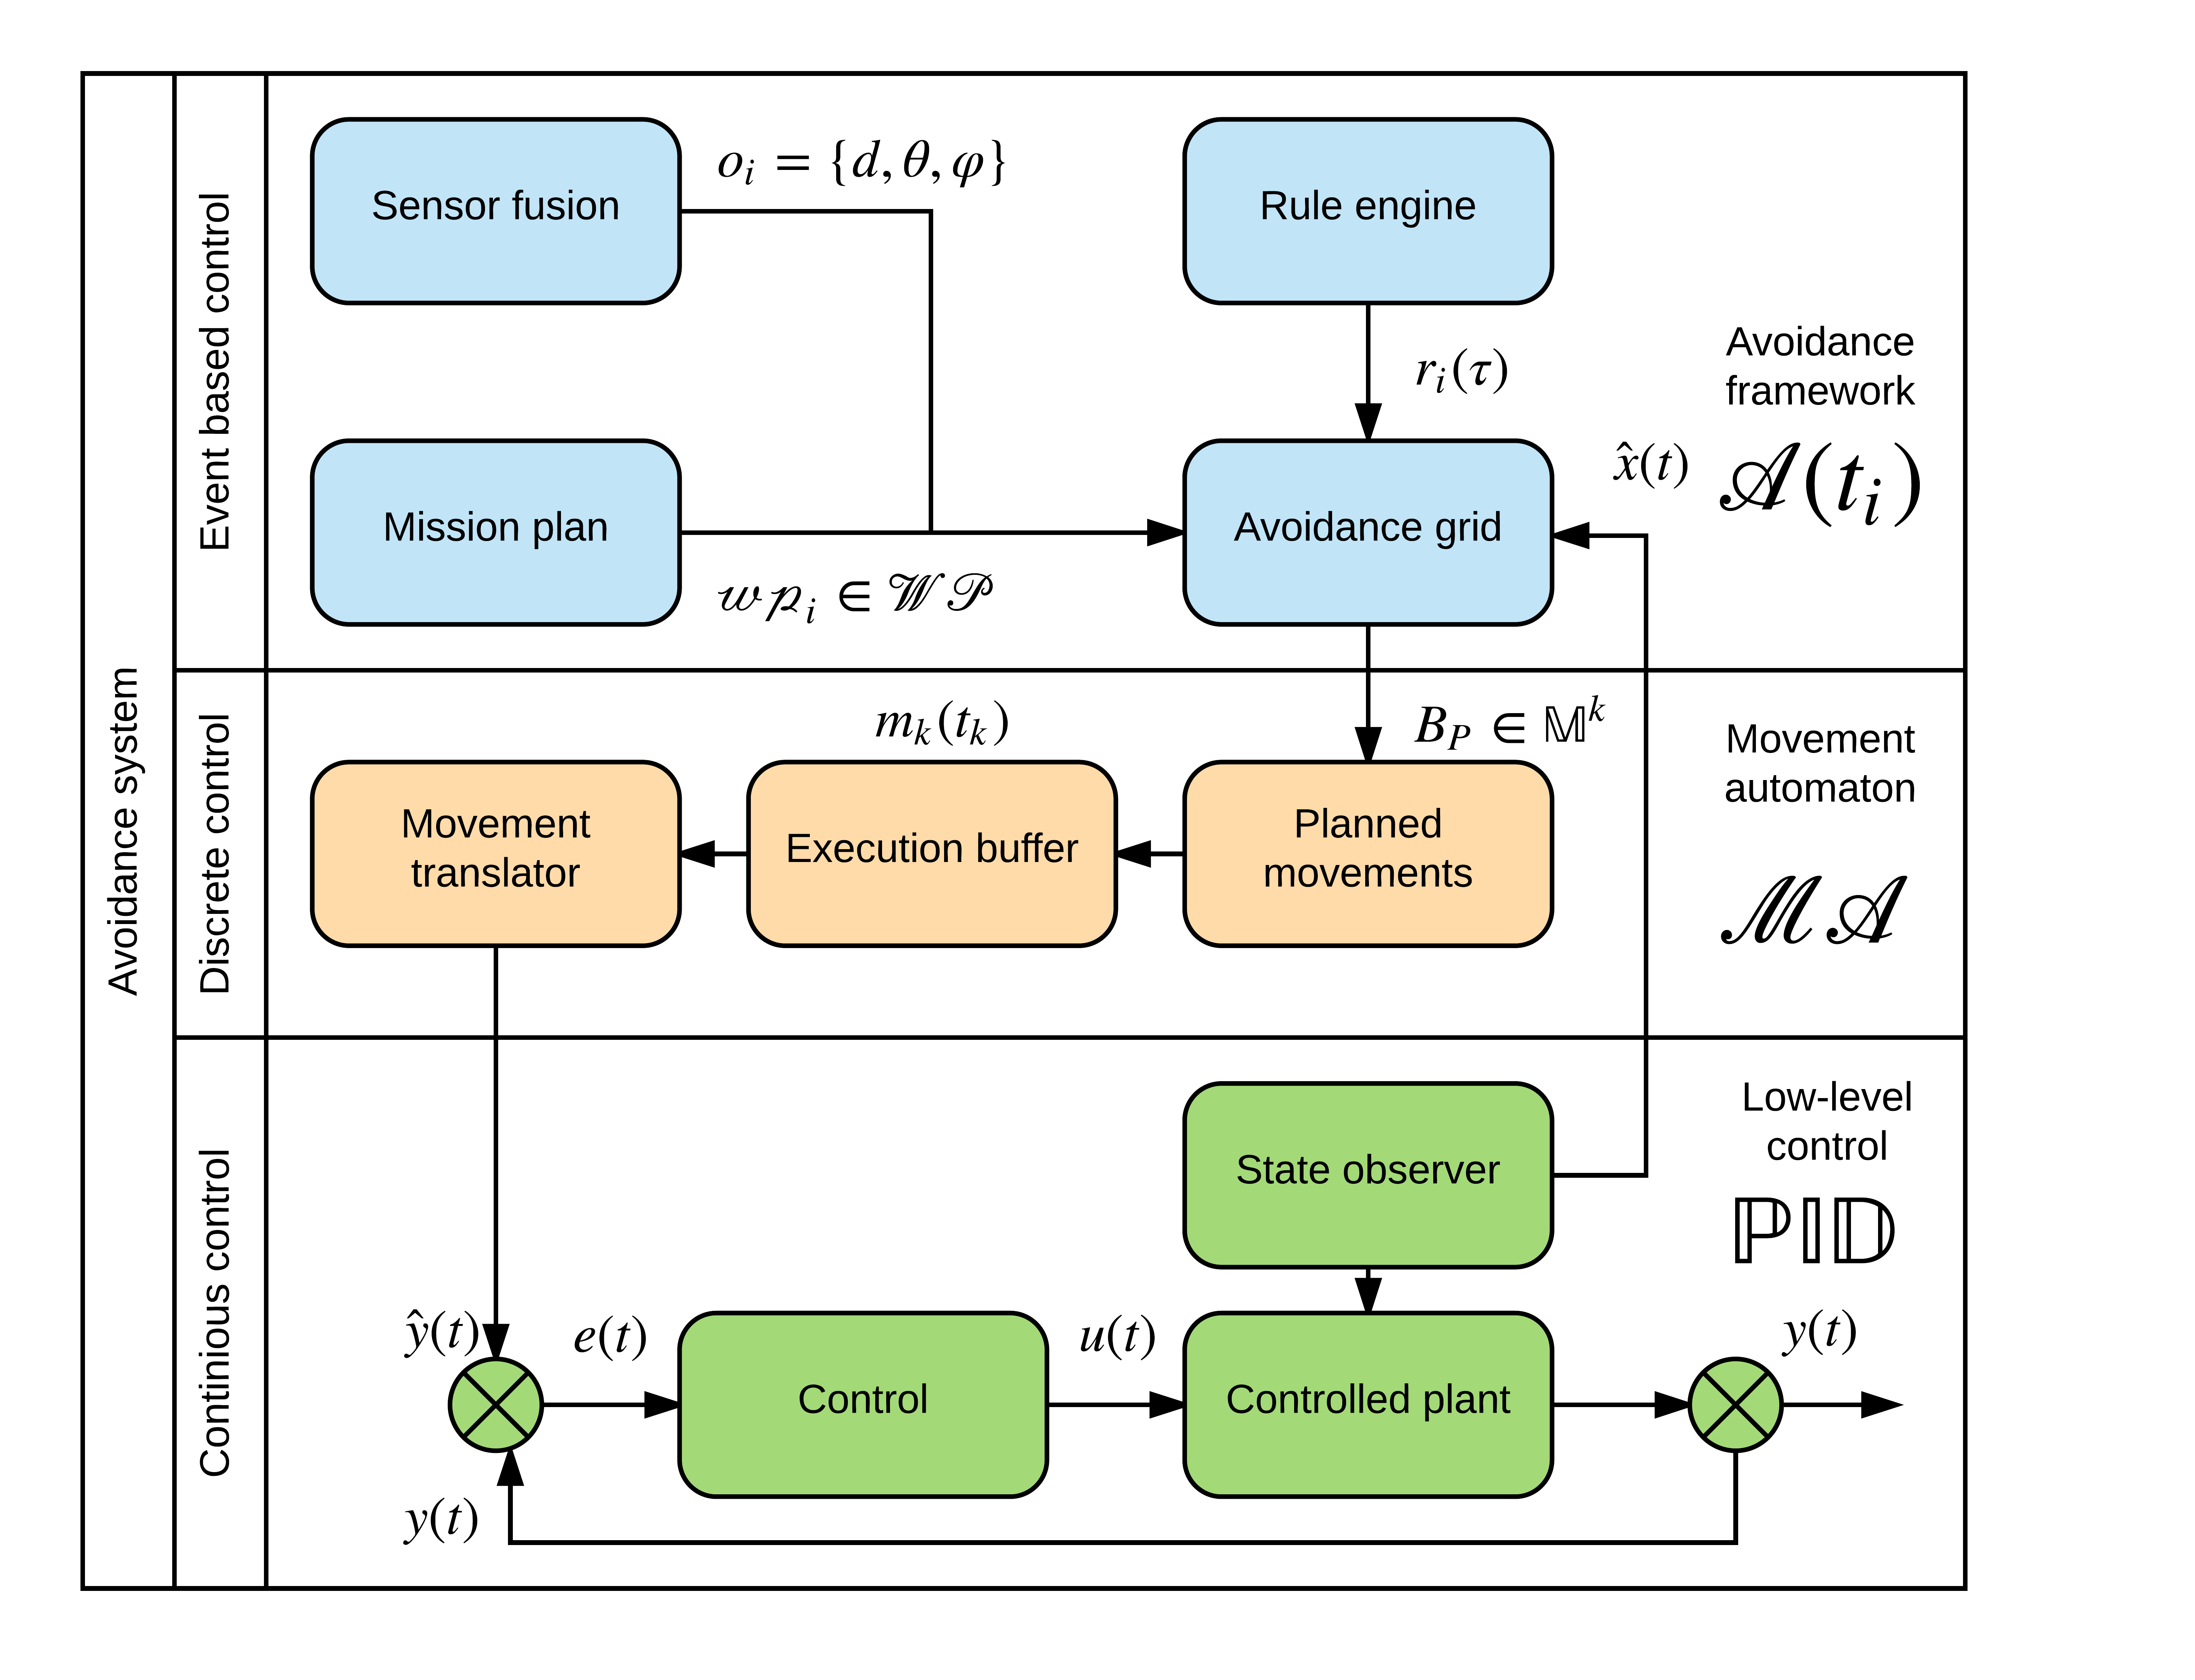
\includegraphics[width=0.8\linewidth]{\FIGDIR/TE001BlockSchemeOfControlConcept} 
    \caption{Obstacle avoidance based on Reach sets concept \cite{gomola2017obstacle}.}
    \label{fig:avoidanceConcept}
\end{figure}

\paragraph{Conceptual scheme:} The overall concept of \emph{Detect and Avoid Framework} (fig. \ref{fig:avoidanceConcept}) is taking architecture from LSTS tool chain \cite{pinto2013lsts,pinto2012implementation}. The UAS part is based on \emph{LSTS Dune} and it can be easily integrated in future. 

\begin{enumerate}
    \item \emph{Continuous control} - is not solved in this work, its kept in scheme for reference. 
    
    \item \emph{Discrete control} - it bridges event based \emph{Detect and Avoid} core functionality with \emph{Continuous control}. Its covered by \emph{Movement Automaton} (sec. \ref{s:movementAutomatonTheory}).

   
    \item \emph{Event based control} - covers major functionalists:    
    \begin{enumerate}[a.]
        \item \emph{Sensor (Data) fusion} - the main feed of information, implementation of \emph{sensor fusion} (sec. \ref{s:SensorFusionDefinition}) and \emph{data fusion} (sec. \ref{s:dataFusionDefinition}) contributing the avoidance events, introduced in (sec. \ref{s:dataFusionProbabilisticModelTheory}).
        
        \item \emph{Mission plan} - feeding actual goal and objectives to \emph{Navigation Algorithm} (sec. \ref{s:NavigationAlgorithms}) and obeying \emph{UTM directives} (sec. \ref{s:utmServicesTheory}).
        
        \item \emph{Avoidance Grid}  - using mainly \emph{Approximation of Reachable Space} (sec. \ref{s:ReachSetEstimationTheory}) in \emph{Avoidance Maneuver Estimation}.
        
        \item \emph{Rule engine} - enforcing UTM directives (sec. \ref{s:utmServicesTheory}).
    \end{enumerate}
    
\end{enumerate}